\documentclass[tikz,border=4pt]{standalone}
\usepackage[T1]{fontenc}
\usepackage[utf8]{inputenc}
\usepackage{FiraSans}
\usepackage{amsmath}
\usetikzlibrary{arrows.meta,positioning,calc}
\definecolor{ceBlue}{RGB}{42,96,153}
\definecolor{ceTeal}{RGB}{36,135,118}
\definecolor{ceGold}{RGB}{220,160,52}
\definecolor{ceRed}{RGB}{188,74,60}
\definecolor{ceInk}{RGB}{42,42,42}
\definecolor{ceGray}{RGB}{238,240,242}
\begin{document}
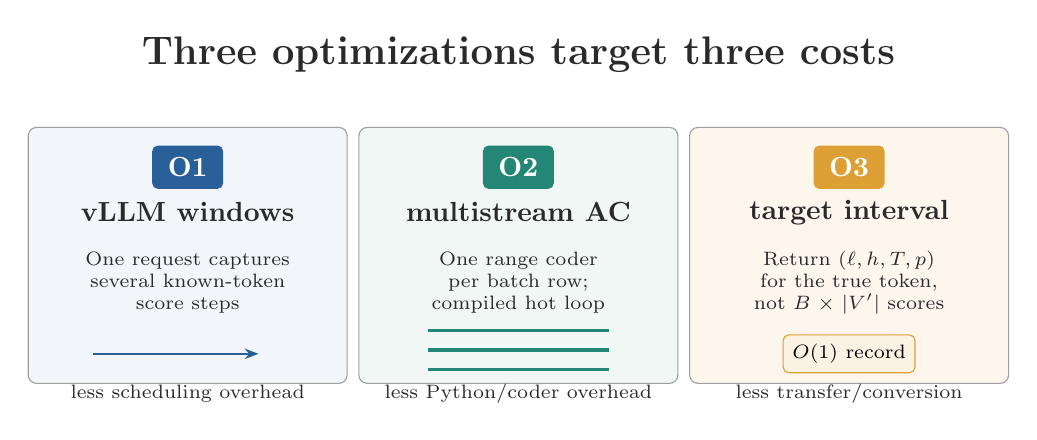
\begin{tikzpicture}[
  x=1cm,y=1cm,
  font=\sffamily,
  card/.style={draw=ceInk!45, rounded corners=3pt, minimum width=4.05cm, minimum height=3.25cm, align=center, fill=white},
  pill/.style={draw=none, rounded corners=2pt, minimum width=0.9cm, minimum height=0.55cm, font=\bfseries, text=white},
  lab/.style={font=\scriptsize, align=center, ceInk},
  arr/.style={-{Stealth[length=5pt]}, thick, ceInk},
]
  \node[font=\Large\bfseries, ceInk] at (6.4,5.55) {Three optimizations target three costs};

  \node[card, fill=ceBlue!6] (o1) at (2.2,3.0) {};
  \node[pill, fill=ceBlue] at (2.2,4.12) {O1};
  \node[font=\bfseries, ceInk] at (2.2,3.55) {vLLM windows};
  \node[lab, text width=3.1cm] at (2.2,2.65) {One request captures\\several known-token\\score steps};
  \draw[arr, ceBlue] (1.0,1.75) -- ++(0.7,0) -- ++(0.7,0) -- ++(0.7,0);
  \node[lab] at (2.2,1.25) {less scheduling overhead};

  \node[card, fill=ceTeal!7] (o2) at (6.4,3.0) {};
  \node[pill, fill=ceTeal] at (6.4,4.12) {O2};
  \node[font=\bfseries, ceInk] at (6.4,3.55) {multistream AC};
  \node[lab, text width=3.2cm] at (6.4,2.65) {One range coder\\per batch row;\\compiled hot loop};
  \foreach \y in {1.55,1.8,2.05} {
    \draw[very thick, ceTeal] (5.25,\y) -- (7.55,\y);
  }
  \node[lab] at (6.4,1.25) {less Python/coder overhead};

  \node[card, fill=ceGold!9] (o3) at (10.6,3.0) {};
  \node[pill, fill=ceGold] at (10.6,4.12) {O3};
  \node[font=\bfseries, ceInk] at (10.6,3.55) {target interval};
  \node[lab, text width=3.2cm] at (10.6,2.65) {Return $(\ell,h,T,p)$\\for the true token,\\not $B\times |V'|$ scores};
  \node[draw=ceGold, rounded corners=2pt, fill=ceGold!14, font=\scriptsize] at (10.6,1.75) {$O(1)$ record};
  \node[lab] at (10.6,1.25) {less transfer/conversion};
\end{tikzpicture}
\end{document}
